\emph{Здесь расписывается архитектура.}

%Подробно расписать, что делает решение. Сделать акцент на том, чем оно отличается от похожих.
%Описать первый блок. Сказать, что природа латентной оптимизации позволяет использовать ее с любой сеткой, но из-за причин был выбран стайлган.
%Описать второй блок. Опять акцент на то, что мы работаем с 2мя фото.

\begin{figure}[h]
\begin{center}
    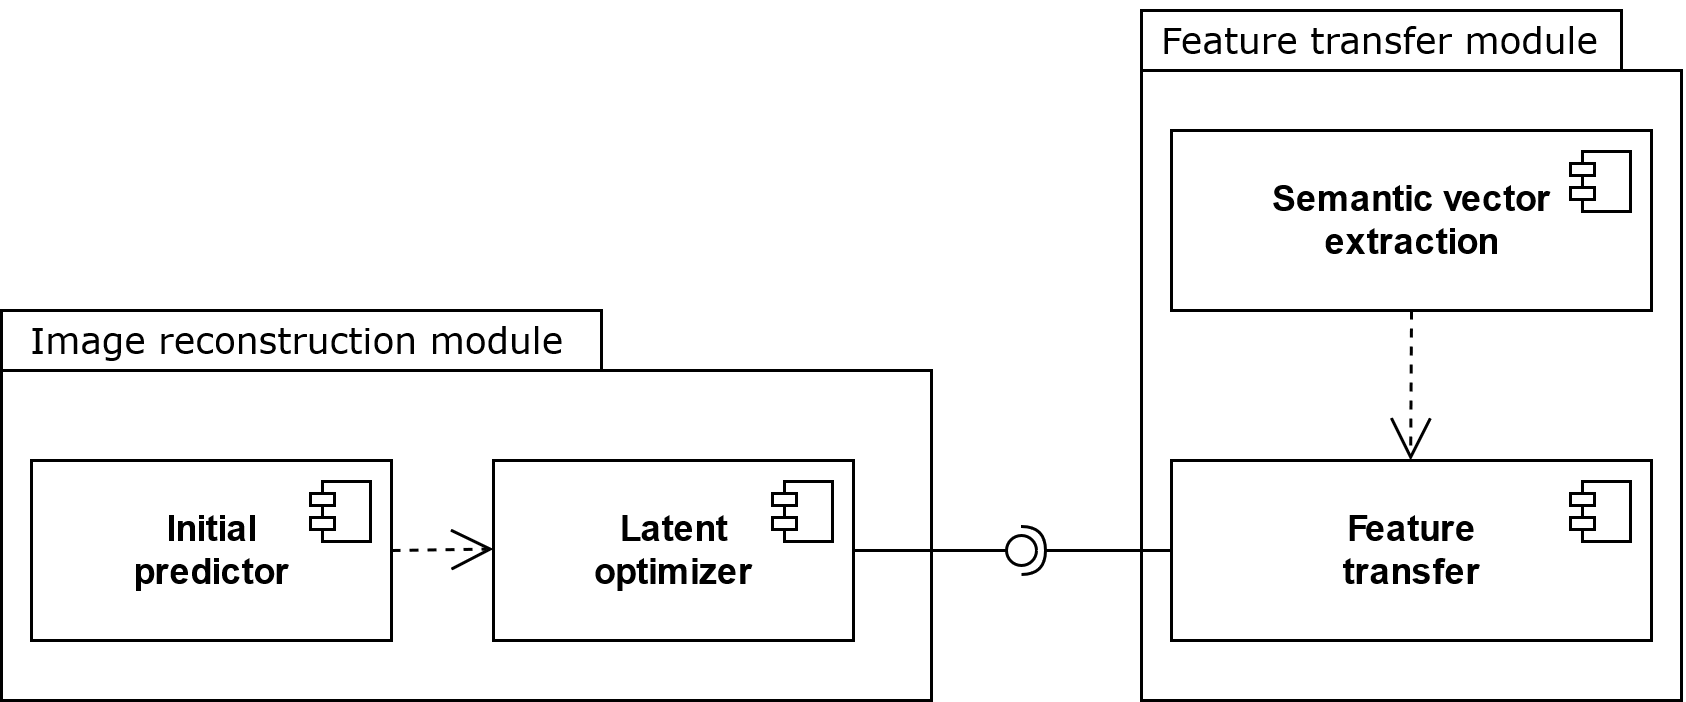
\includegraphics[width=0.9\textwidth]{Architecture_eng}
    \caption{Архитектура решения (\emph{Диаграмма в процессе работы, GAN-ы отдельно не надо, потому что композиция, и они часть компонента, в feature transfer добавить выделение фич}).}
    \label{fig:architecture}
\end{center}
\end{figure}

В рамках данной работы было разработано решение для семантического редактирования изображений. Это решение позволет редактировать изображения лиц в терминах высокоуровневых лицевых признаков, нитуитивно понятных человеку. %таких как положение головы, наличие улыбки и т.д.
% с двумя режимами работы: 1) по предоставленному методу разметки выделить семантический признак в латентном пространстве сети, 2) ...
По двум входным изображениям, целевому изображению и изображению-образцу, это решение способно произвести перенос заданного лицевого признака с изображения-образца на целевое изображение.
Решение способно работать с произвольными бинарными признаками, но ...
%Для неизвестного признака решение может что -то зделать, если передана процедура разметки/Чтобы добавить новый признак

Решение состоит из двух функциональных частей: модуля реконструкции изображения (?в латентном пространстве генеративной состязательной сети), и модуля семантического редактирования (?в латентном пространстве сети).

Первый модуль осуществляет отображение входных изображений в латентное пространство имеющейся генеративной состязательной сети, т.е. находит такой латентный вектор, с помощь которого генератор имеющейся генеративной состязательной сети сгенерирует максимально похожее изображение.
% он включает в себя компонент1 и компонент2 (?)
% он производит гибридный метод латентной оптимизации (отсылаемся к обзору), энкодер предсказывает начальное приближение, потом непосредственная оптимизация латентного вектора.
%Здесь пишем что это в.т.ч. для артист-контроля, позволяет быстро получить отклик для пользователя, и при этом дать гибкий контроль между затраченным временем и полученной точностью.

Второй модуль осуществляет манипулирование полученными латентными представлениями. Этот модуль отвечает за выявление преобразования в латентном пространстве, соответствующего заданному лицевому признаку, а также за процесс переноса заданного признака с изображения образца на целевое изображение.
% он включает в себя компонент3 и компонент4
% здесь пишем про то, что для выделения семантик нужна процедура разметки (или выборка положительных/отрицательных примеров), а также про то, что мы вводим нелинейность для сохранения личности?

%Оба модуля взаимодействуют с пользователем посредством веб—интерфейса.